% The resolution cascade for a single column: the first tier that can produce a
% constraint-valid value wins, and the last tier can never decline.
\documentclass[tikz,border=6pt]{standalone}
% Shared preamble for all standalone paper figures.
% Palette and TikZ setup carried over from the legacy generator
% (paper/figures/scripts/build_paper_figures.py, TIKZ_HEADER) so the new
% figures keep the established visual identity.
\usepackage[T1]{fontenc}
\usepackage{amssymb}
\usepackage{helvet}
\renewcommand{\familydefault}{\sfdefault}
\usepackage{tikz}
\usepackage{pgfplots}
\pgfplotsset{compat=1.18}
\usetikzlibrary{arrows.meta,positioning,fit,calc,shapes.geometric}

\definecolor{mockblue}{HTML}{2E6F9E}
\definecolor{mockgreen}{HTML}{4F8A70}
\definecolor{mockred}{HTML}{C0392B}
\definecolor{mockgold}{HTML}{B08A2E}
\definecolor{mockgray}{HTML}{F4F1EC}
\definecolor{mockink}{HTML}{2B2B2B}

\tikzset{
  box/.style={draw=mockink!60, fill=white, rounded corners=2pt, align=center,
    inner sep=5pt, font=\small},
  main/.style={box, fill=mockgray, draw=mockink!70, thick},
  tzero/.style={box, fill=mockblue!14, draw=mockblue, thick},
  tone/.style={box, fill=mockgreen!14, draw=mockgreen, thick},
  ttwo/.style={box, fill=mockgold!16, draw=mockgold, thick},
  tthree/.style={box, fill=mockred!12, draw=mockred, thick},
  decision/.style={draw=mockink!70, fill=white, diamond, aspect=2.2,
    align=center, inner sep=2pt, font=\small},
  chip/.style={draw, rounded corners=4pt, inner sep=2.5pt, font=\scriptsize\bfseries,
    text=white},
  chipzero/.style={chip, fill=mockblue, draw=mockblue},
  chipone/.style={chip, fill=mockgreen, draw=mockgreen},
  chiptwo/.style={chip, fill=mockgold, draw=mockgold},
  chipthree/.style={chip, fill=mockred, draw=mockred},
  arrow/.style={-{Stealth[length=2.6mm]}, thick, mockink!80},
  yes/.style={arrow, mockgreen!80!black},
  no/.style={arrow, mockred!70!black},
  note/.style={font=\scriptsize, text=mockink!75, align=center},
  banner/.style={draw=mockink!70, fill=mockgray, rounded corners=3pt,
    align=center, inner sep=6pt, font=\small\bfseries},
}

\begin{document}
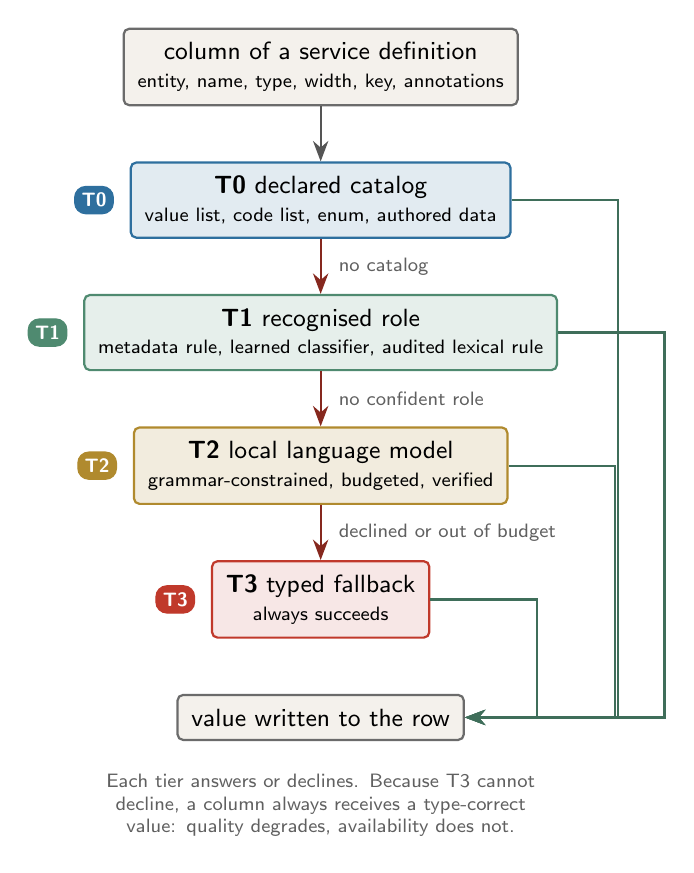
\begin{tikzpicture}[node distance=5mm]

\node[main] (field) {column of a service definition\\[-1pt]
  {\scriptsize entity, name, type, width, key, annotations}};

\node[tzero, below=7mm of field] (t0) {\textbf{T0} declared catalog\\[-1pt]
  {\scriptsize value list, code list, enum, authored data}};
\node[tone, below=7mm of t0] (t1) {\textbf{T1} recognised role\\[-1pt]
  {\scriptsize metadata rule, learned classifier, audited lexical rule}};
\node[ttwo, below=7mm of t1] (t2) {\textbf{T2} local language model\\[-1pt]
  {\scriptsize grammar-constrained, budgeted, verified}};
\node[tthree, below=7mm of t2] (t3) {\textbf{T3} typed fallback\\[-1pt]
  {\scriptsize always succeeds}};

\node[main, below=7mm of t3] (out) {value written to the row};

\draw[arrow] (field) -- (t0);
\draw[no] (t0) -- node[note, right=1mm] {no catalog} (t1);
\draw[no] (t1) -- node[note, right=1mm] {no confident role} (t2);
\draw[no] (t2) -- node[note, right=1mm] {declined or out of budget} (t3);

\foreach \tier/\chip in {t0/chipzero, t1/chipone, t2/chiptwo, t3/chipthree} {
  \draw[yes] (\tier.east) -- ++(1.35,0) |- (out.east);
}

\node[chipzero, left=2mm of t0] {T0};
\node[chipone, left=2mm of t1] {T1};
\node[chiptwo, left=2mm of t2] {T2};
\node[chipthree, left=2mm of t3] {T3};

\node[note, below=3mm of out, text width=62mm]
  {Each tier answers or declines. Because T3 cannot decline, a column always
   receives a type-correct value: quality degrades, availability does not.};

\end{tikzpicture}
\end{document}
